\glsresetall
\chapter{API Usability Analyzer}
\label{app:apiua}

Dieser Teil vertieft die Erläuterungen zu Entwurfsentscheidungen und Komponenten des \gls{apiua}.

\section{Services}
\label{sec:services}

\subsection*{LocatorService}

Dieser Dienst ist dafür zuständig, \glslink{uri}{URIs} aufzulösen, zu laden und als Objekt bereitzustellen. Dazu wird --- neben vielen Varianten --- die Methode \mintinline{java}{<T extends ILocatable> Future<T> resolve(final URI uri, final Class<T> clazz, final IProgressMonitor monitor)} bereitgestellt. Die Erzeugung mancher Objekte kann viel Zeit in Anspruch nehmen. Daher wird diese Operation stets in einem separaten Thread ausgeführt und der Fortschritt innerhalb von \gls{apiua} durch eine Fortschrittsleiste dargestellt.

Sobald das zu suchende Objekt konstruiert wurde, kann darauf mittels \mintinline{java}{Future<T>.get()} zugegriffen werden. Diese Methode gibt \texttt{null} zurück, wenn das Objekt nicht existiert oder nicht zuweisungskompatibel zur übergebenen Klasse ist.

Der LocatorService verwendet intern einen Cache, der die Objekte verdrängt, auf die am seltensten zugegriffen wurde.

\subsection*{DataService}

Dieser Dienst kapselt die Funktionalität, die zur Verwaltung von Datenverzeichnissen notwendig ist. Ein Datenverzeichnis enthält dabei alle, zu einem Ereignis aufgezeichneten Daten. Solche Daten können Programmierfortschritte, Gruppendiskussion, etc. sein.

Ein Datenverzeichnis wird durch eine Instanz des \texttt{IBaseDataContainer}-Interfaces dargestellt. Unterverzeichnisse implementieren das Interface \texttt{IDataContainer} und enthalten die eigentlichen \texttt{IData}-implementierenden Daten.

Die Daten werden vollständig von ihrer Speicherform abstrahiert. Aktuell gibt es eine Implementierung für Dateisysteme (\texttt{FileBaseDataContainer}, \texttt{FileDataContainer}, \texttt{FileData}). Es wären aber auch Implementierungen für den Zugriff auf Datenbanken, etc. möglich.

Eine weitere Aufgabe des DataService besteht im Laden von Datenverzeichnissen. Der Lademechanismus ist deklarativ erweiterbar. Gibt es beispielweise ein Plugin, das Daten vom Typ \texttt{A} laden kann und auf geladene Daten vom Typ \texttt{B} eines anderen Plugins angewiesen ist, fordert DataService erst den Ladeprozess für \texttt{B} und dann für \texttt{A} an. Datenformate, die untereinander keine Abhängigkeiten aufweisen, werden parallel geladen. Mehr Informationen zu Datentyp-Plugins finden sich im \sref{sec:schicht3}.

\subsection*{CodeService}

Der CodeService wird durch das \acrshort{gtm}-Plugin (siehe \fref{fig:apiua-plugins}) bereitgestellt. Seine Aufgabe besteht darin, das Erstellen, Lesen, Editieren und Löschen von Kodes, Kodeinstanzen, Relationen, Relationsinstanzen, \glspl{acm}, \glspl{ac}, Memos, etc. zu ermöglichen.

Die Implementierung basiert im Wesentlichen auf zwei Entwurfsentscheidungen, die weiter unten ausführlicher beschrieben sind:
\begin{enumerate}
  \item Die Datenhaltung selbst ist in die Klasse \texttt{CodeStore} ausgelagert. CodeService kapselt diese Klasse und ist für die Invariantenprüfung zuständig.
  \item Die Verwendung spezieller Caches vermeidet unnötige mehrfache Berechnungen.
\end{enumerate}

\paragraph{Datenhaltung}

CodeService verwendet zur Speicherung seiner Daten die CodeStorage-Klasse. Sie speichert und lädt Daten ohne eine Invariante zu haben oder gar zu prüfen. So kann beispielswiese eine Kodeinstanz auf einen nicht mehr existierenden Kode zeigen. Diese Prüfung wird vom CodeService selbst übernommen.

Der CodeStore speichert mit zwei Ausnahmen alle Daten in einer XML-Datei. Ein beispielhafter \texttt{CodeStore.xml} könnte wie folgt aussehen:

\begin{center}
\begin{minted}[linenos, firstnumber=1, autogobble=false]{xml}
<codeStore>
  <createdIDs class="sorted-set">
    <long>-9223372036854775808</long>
    <long>-9223372036854775807</long>
    <long>-9223372036854775806</long>
\end{minted}
\texttt{...}
\begin{minted}[linenos, firstnumber=5428, autogobble=false]{xml}
                <com.bkahlert.nebula.data.TreeNode>
                  <parent reference="../../.."/>
                  <children/>
                  <data class="codes">
                    <uri>apiua://code/-9223372036854775633</uri>
                    <id>-9223372036854775633</id>
                    <caption>Inkonsistenzen bzgl. STD/STL</caption>
                    <color>
                      <red>0.22499999999999998</red>
                      <green>0.775</green>
                      <blue>0.396875</blue>
                      <alpha>1.0</alpha>
                    </color>
                    <creation>
                      <calendar>
                        <time>1364917869690</time>
                        <timezone>Europe/Berlin</timezone>
                      </calendar>
                    </creation>
                  </data>
                </com.bkahlert.nebula.data.TreeNode>
\end{minted}
\texttt{...}
\begin{minted}[linenos, firstnumber=7549, autogobble=false]{xml}
    <instance>
      <uri>apiua://codeinstance/-9223372036854775765</uri>
      <codeInstanceId>-9223372036854775765</codeInstanceId>
      <code class="codes" reference="[...]nebula.data.TreeNode[3]/data"/>
      <id>apiua://diff/0meio6dzt3eo1wj7/16/sandbox%2Fmy_sandbox%2F apps%2Fmy_app%2Fmy_app.cpp</id>
      <creation>
        <calendar>
          <time>1343386987000</time>
          <timezone>Europe/Berlin</timezone>
        </calendar>
      </creation>
    </instance>
\end{minted}
\texttt{...}
\begin{minted}[linenos, firstnumber=15311, autogobble=false]{xml}
    <relations>
      <uri>apiua://relation/293gbmficnukqqg68ihv7atasdtc0rf7</uri>
      <from reference="[...]nebula.data.TreeNode[18]/data/uri"/>
      <to reference="[...]nebula.data.TreeNode[2]/data/uri"/>
      <name>bedingt</name>
      <timeZoneDate>
        <calendar>
          <time>1418791813845</time>
          <timezone>Europe/Berlin</timezone>
        </calendar>
      </timeZoneDate>
    </relations>
\end{minted}
\texttt{...}
\begin{minted}[linenos, firstnumber=23431, autogobble=false]{xml}
</codeStore>
\end{minted}
\captionof{listing}[Beispiel: CodeStore.xml]{Auszug aus der CodeStore.xml, auf der diese Arbeit basiert.}
\label{lst:codestore-file}
\end{center}

Memos und \glspl{acm} werden in separaten Dateien gespeichert. Jede einzelne Memo wird in einer HTML-Datei gespeichert, deren Name der \gls{uri} des Objekts entspricht, zu dem diese Memo gehört. Ein \gls{acm} wird in einer JSON-formatierten Datei gespeichert, die wie folgt aussehen kann:

\begin{center}
\begin{minted}[linenos, firstnumber=1, autogobble=false]{json}
{
  "cells":[
    {
      "type":"html.Element",
      "position":{
        "x":-885,
        "y":1198
      },
      "size":{
        "width":128,
        "height":28
      },
      "angle":0,
      "id":"apiua://code/-9223372036854775552",
      "title":"Performance<div class=\"details\">[...]</div>",
      "content":"",
      "z":0,
      "customClasses":[

      ],
      "color":"rgb(255, 255, 255)",
      "background-color":"rgb(163, 198, 57)",
      "border-color":"rgb(138, 168, 49)",
      "attrs":{

      }
    },
\end{minted}
\texttt{...}
\begin{minted}[linenos, firstnumber=679, autogobble=false]{json}
    {
      "type":"link",
      "source":{
        "id":"apiua://code/-9223372036854775623"
      },
      "target":{
        "id":"apiua://code/-9223372036854775440"
      },
      "labels":[
        {
          "position":0.5,
          "attrs":{
            "text":{
              "text":"bedingt\n3 (2)"
            }
          }
        }
      ],
      "id":"apiua://relation/hjg2ikddvbh1nrj9uc646kjr1uf6agha",
      "smooth":true,
      "z":28,
      "customClasses":[

      ],
      "vertices":[
        {
          "x":370.25,
          "y":1741
        }
      ],
      "attrs":{
        ".marker-target":{
          "d":"M 10 0 L 0 5 L 10 10 z"
        }
      }
    }
\end{minted}
\texttt{...}
\begin{minted}[linenos, firstnumber=2811, autogobble=false]{json}
  {
    "title":"Wiederverwendbarkeit von Wissen: OOP- und STL-Inkonsistenten",
    "zoom":0.8000000000000005,
    "pan":{
      "x":-66.08609376562507,
      "y":-1103.5950979062497
    }
  }
\end{minted}
\texttt{...}
\captionof{listing}[Beispiel: ACM-Datei]{Auszug aus der JSON-formatierten ACM-Datei \texttt{acm.apiua\%3A\%2F\%2Faxialcodingmodel\%2FQpPaMj4mceVnuSYI}}
\label{lst:acm-file}
\end{center}

\paragraph{Cache}

Im \sref{sec:gtm-implementation} wird ausführlich beschrieben, dass \gls{apiua} über fest implementierte Interferenzregeln verfügt. Der CodeService ist der Ort, an dem die dazu notwendigen Daten (z.B. hypothetische Relationen) berechnet werden. Diese Berechnung muss sehr effizient vonstatten gehen, da jede Theoriemodelländerung, Teile dieser Berechnungen ungültig macht.

Dazu wurde eine \textit{DataCache}-Klasse implementiert, die Berechnungen auf der Grundlage ihrer Eingabedaten abstellt und zwischenspeichert. Die Berechnung findet nur dann, wenn die Ergebnisse überhaupt erfragt werden und sich die zugrunde liegenden Daten verändert haben.

Im Laufe meiner Forschung mit \gls{apiua} musste ich feststellen, dass die Anwendung extrem langsam geworden ist. Grund dafür war die Einführung der Interferenzregeln, deren Anwendung auf das vom mir generierte Theoriemodell viel Zeit kostete. Jede Anfrage löste eine erneute Berechnung aus.

Der Einsatz der DataCache-Klasse löste das Problem. Nun gibt es vier DataCache-Erben (\textit{CodeCache}, \textit{CodeInstanceCache}, \textit{RelationCache}, \textit{RelationInstanceCache}), die auf Teilen des Theoriemodells arbeiten (\textit{CodeCache} nutzt den Kodebaum als Eingabe) und durch Abhängigkeiten untereinander eine Baumstruktur bilden (\textit{CodeInstanceCache} nutzt als Eingabe die Liste der KodeInstanzen und den \textit{CodeCache}). Dieser Ansatz führt dazu, dass nur Teile der Interferenzberechnungen im Falle einer Änderung am Theoriemodell neu berechnet werden müssen. Die nun zwischengespeicherten Ergebnisse erfordern keine ständige Neuberechnung mehr.

Ursprünglich erkannte die \textit{DataCache}-Klasse Änderungen an seinen Eingaben mit Hilfe der \texttt{hash}-Funktion. Diese Implementierung wurde allerdings auf eine explizite Methode (\texttt{DataView.setLastModification(long nanoseconds)}) umgestellt, da die Änderung des hash-Werts keine Aussage darüber zulässt, ob sich das Objekt im Auge des Entwicklers hinreichend verändert hat und damit einer Neuberechnung bedarf.



\subsection*{LabelProviderService}

Dieser Dienst erlaubt es, die Bezeichner, Icons, etc. von Objekten in Erfahrung zu bringen, die durch andere Plugins beigesteuert werden. Möchte zum Beispiel eine Ansicht alle Verankerungen einer bestimmten Relation darstellen, können diese mittels \mintinline{java}{Set<IRelationInstance> ICodeService.getExplicitRelationInstances(IRelation relation)} erfragt werden. Die Phänomene werden mit Hilfe von \mintinline{java}{URI IRelationInstance.getPhenomenon()} ermittelt. Da die Phänomene möglicherweise selbst nicht geladen sind, werden sie lediglich durch eine \gls{uri} identifiziert.

Um nun Daten unbekannter Quelle, darstellen zu können, kann auf die Methoden \mintinline{java}{StyledString getStyledText(URI uri)}, \mintinline{java}{String getText(URI uri)} und \mintinline{java}{getImage(URI uri)} zugegriffen werden. Der LabelProviderService delegiert die Anfragen dann an den zuständigen LabelProvider und gibt den Bezeichner bzw. das Icon zurück.

Im \sref{sec:schicht3} wurde bereits beschrieben, dass jedes Datentyp-Plugin einen LabelProvider bereitstellen muss, der die Anzeigeinformationen  für die Daten berechnen kann, für die das Plugin zuständig ist.



\section{Browser}
\label{sec:browser}

Das \gls{swt} stellt einen Wrapper und damit eine standardisierte Schnittstelle für den plattformabhängigen Standard-Webbrowser bereit. Seine Kernfunktionalität besteht im Laden von Webseiten und in der Möglichkeit, von \gls{java} aus JavaScript-Code innerhalb des Browsers auszuführen. Der \gls{swt}-Browser sollte ursprünglich als Grundlage für die \acrshort{ui}-Komponenten von \gls{apiua} dienen. Leider war das Funktionsspektrum zu eingeschränkt, um es problemlos für die auf Websprachen basierte \acrshort{ui}-Entwicklung zu verwenden.

Ich habe das von mir entwickelte \textit{Nebula}-\gls{plugin}\footnote{\url{https://github.com/bkahlert/com.bkahlert.nebula}} um eine Browser-Komponente erweitert, um die Unzulänglichkeiten des \acrshort{swt}-Browsers zu beheben.

Einen Browser für die Implementierung von Benutzeroberflächen zu verwenden, hat den Vorteil, die extrem hohe Performanz aktueller Browser nutzen zu können. Darüber existiert eine Unmenge an wiederverwendbaren auf Websprachen basierten Lösungen für verschiedenste Probleme. \autoref{fig:BrowserEditor} zeigt eine auf einen Browser basierende \acrshort{ui}-Komponente, die einen Rich-Text-Editor bereitstellt. \autoref{fig:BrowserColors} veranschaulicht, wie das Funktionsspektrum der \textit{Nebula}-Utility-Klasse \textit{ColorUtils} mit Hilfe des \textit{Nebula}-Browser dargestellt wird.

\begin{figure}
  \centering
    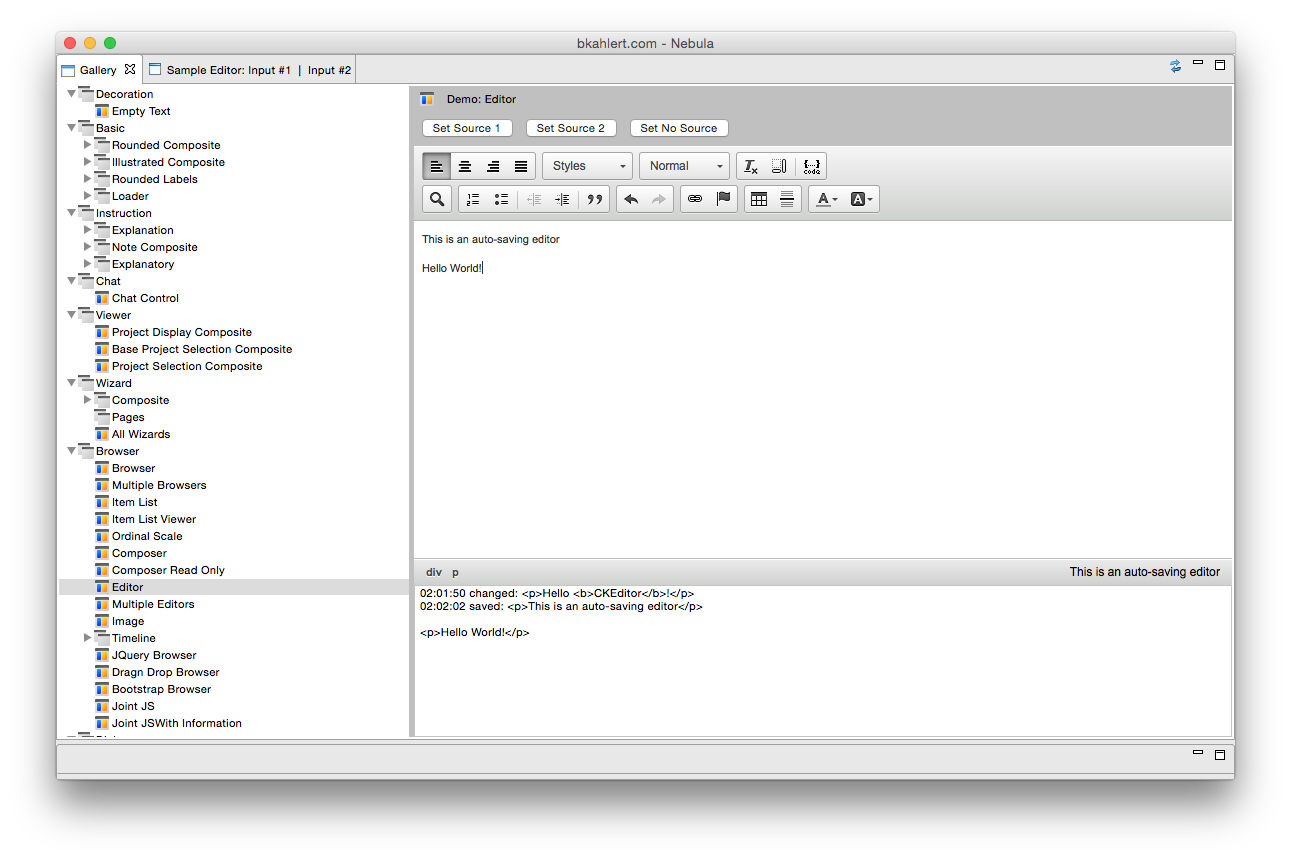
\includegraphics[width=1.0\linewidth]{Figures/browser/BrowserEditor.png}
  \caption[Nebula-Browser-basierter Rich-Text-Editor]{Im rechten Bereich der \textit{Widget Gallery} wird ein auf dem \textit{Nebula}-Browser basierender Rich-Text-Editor dargestellt. Er verwendet den Open-Source-Web-Editor \textit{CKEditor} (\url{http://ckeditor.com}).}
  \label{fig:BrowserEditor}
\end{figure}

\begin{figure}
  \centering
    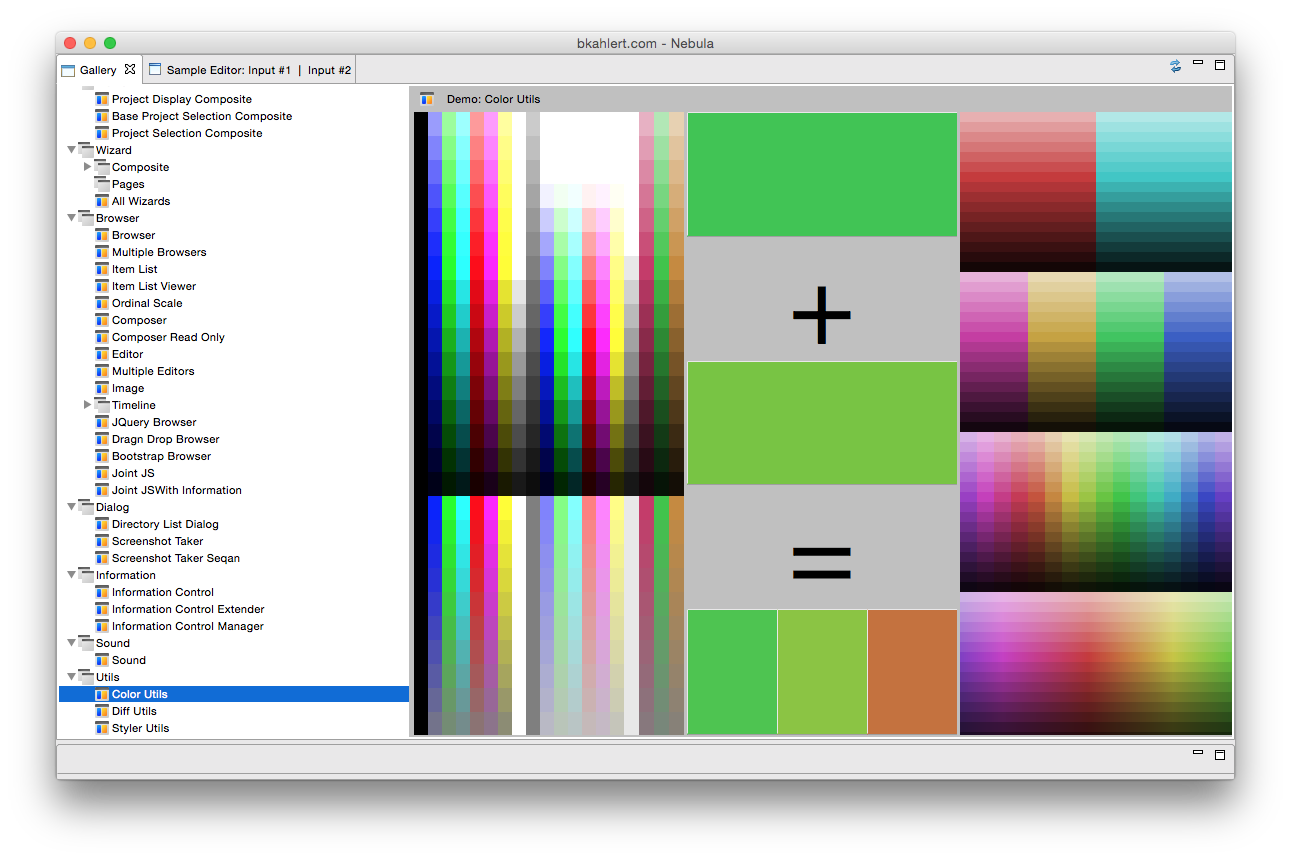
\includegraphics[width=1.0\linewidth]{Figures/browser/BrowserColors.png}
  \caption[Nebula-Browser: Veranschaulichung einer Utility-Klasse]{Im rechten Bereich der \textit{Widget Gallery} wird eine auf dem \textit{Nebula}-Browser basierende Funktionsdemonstration der \textit{Nebula}-Utility-Klasse dargestellt.}
  \label{fig:BrowserColors}
\end{figure}



Weiterer Bestandteil des \textit{Nebula}-\gls{plugin}s ist die \textit{Widget Gallery}. Sie stellt alle vom \textit{Nebula}-\gls{plugin} bereitgestellten \acrshort{ui}-Komponenten in verschiedenen Konfigurationen dar. Sie dient damit einerseits als Überblick und andererseits als Dokumentation der Verwendungsweise der vorhandenen \acrshort{ui}-Komponenten.

Die Abbildungen \ref{fig:BrowserEditor}, \ref{fig:BrowserColors}, \ref{fig:BrowserExternal}, \ref{fig:BrowserList} und \ref{fig:BrowserDND} zeigen, wie die verschiedenen Anwendungen der Browser-Komponenten in der Widget Gallery dargestellt werden.

Der \textit{Nebula}-Browser kapselt den \gls{swt}-Browser und unterscheidet sich von diesem wie folgt:

\begin{description}
  \item[Erweiterungen] \hfill \\
  Eine in dem Browser geladene Seite kann erweitert werden. Erweiterungen bestehen aus einer beliebigen Anzahl von CSS- und JavaScript-Dateien. Erweiterungen können Abhängigkeiten zu anderen Erweiterungen definieren, die im Falle ihrer Abwesenheit automatisch geladen werden. Außerdem wird sichergestellt, dass eine Erweiterung maximal einmal geladen wird. Durch Erweiterungen können beispielsweise Bibliotheken wie jQuery\footnote{\url{http://jquery.com}} nachgeladen werden. 
  
  \autoref{fig:BrowserExternal} zeigt, wie auf diese Weise die Hintergrundfarbe von \url{wikipedia.org} geändert werden kann. \autoref{fig:BrowserList} hingegen zeigt eine Reihe von Knöpfen, deren Gestalt und Verhalten durch das Laden des \textit{Bootstrap-Frameworks} verändert wurde.
  
  \begin{figure}
    \centering
      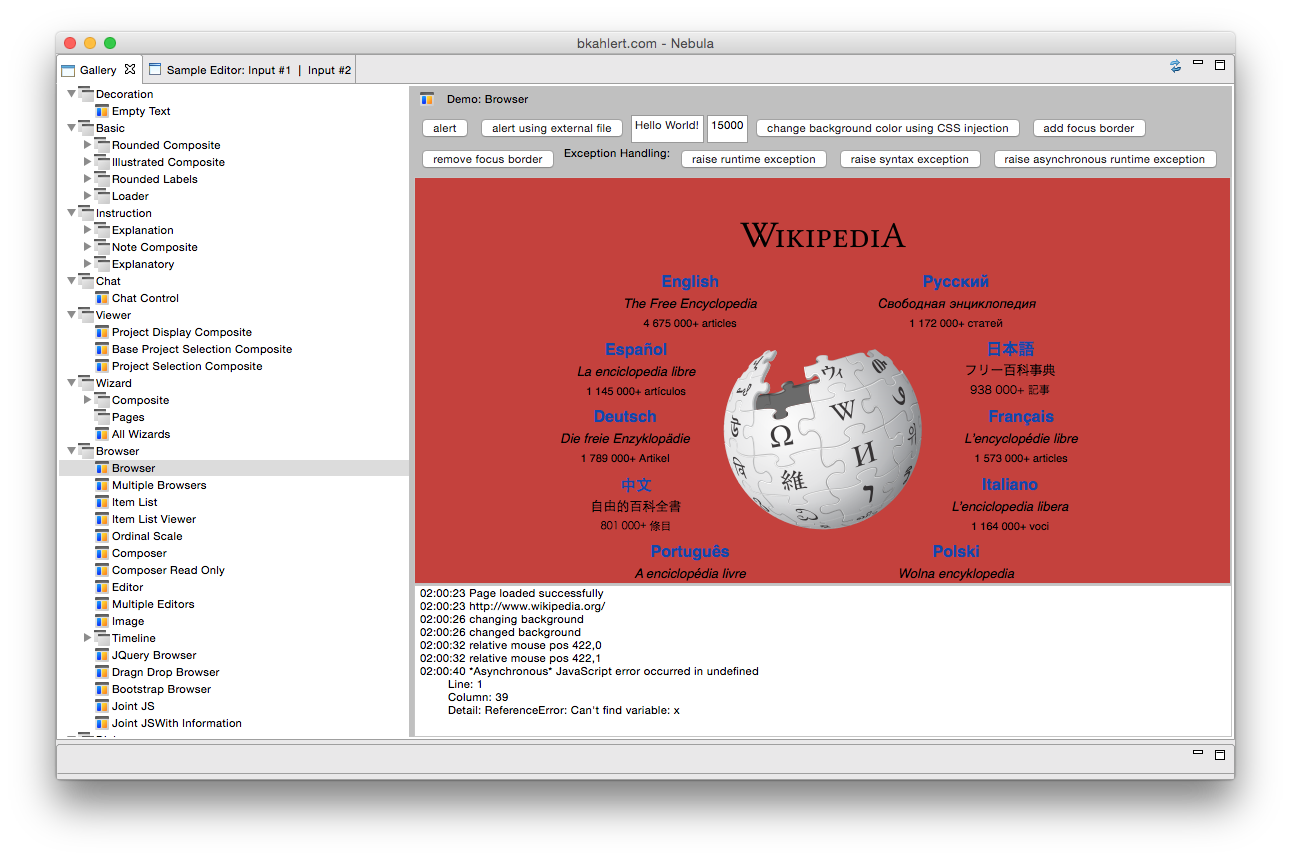
\includegraphics[width=1.0\linewidth]{Figures/browser/BrowserExternal.png}
    \caption[Nebula-Browser mit geladener Wikipedia-Startseite]{Im rechten Bereich der \textit{Widget Gallery} wird ein \textit{Nebula}-Browser dargestellt, der mittels einer Erweiterung die Hintergrundfarbe der geladenen Wikipedia-Startseite ändert. In dem darunter liegenden Verlauf, wird gezeigt, wie eine testweise geworfene Ausnahme gefangen wurde.}
    \label{fig:BrowserExternal}
  \end{figure}
  
  \begin{figure}
    \centering
      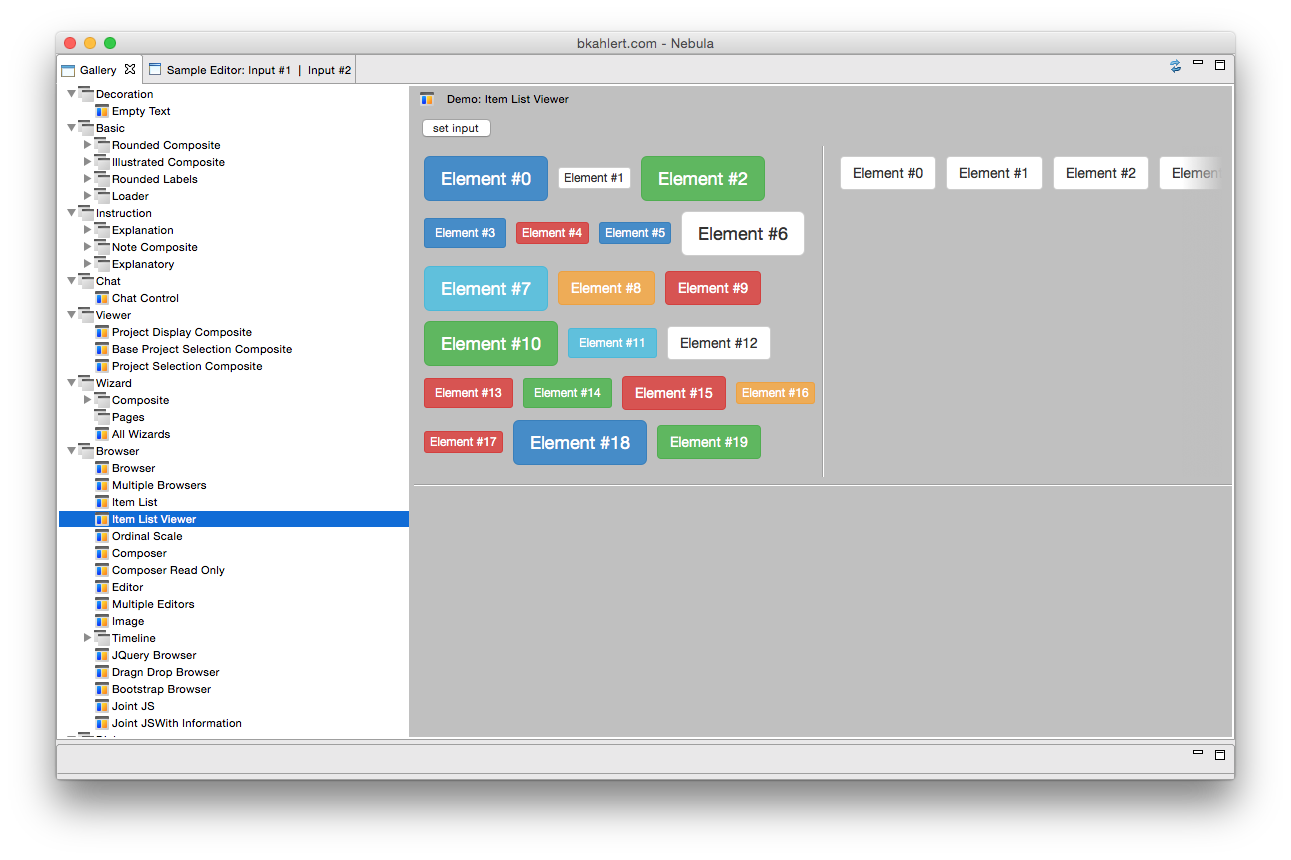
\includegraphics[width=1.0\linewidth]{Figures/browser/BrowserList.png}
    \caption[Nebula-Browser mit Bootstrap-Erweiterung]{Im rechten Bereich der \textit{Widget Gallery} werden zwei \textit{Nebula}-Browser dargestellt, die mit Hilfe des \textit{Bootstrap-Frameworks} (\url{http://getbootstrap.com}) erweiterte Knöpfe darstellen.}
    \label{fig:BrowserList}
  \end{figure}
  
  Der Lebenszyklus ist ausdifferenziert. Die folgenden Methoden können überschrieben werden: \texttt{beforeLoad}, \texttt{afterLoad}, \texttt{beforeCompletion}, \texttt{afterCompletion}, \texttt{scriptAboutToBeSentToBrowser}, \texttt{scriptReturnValueReceived} und \texttt{dispose}.
  
  \item[Asynchrone Schnittstelle] \hfill \\
  \gls{swt} erzwingt, dass Code, der mit einer \acrshort{ui}-Komponente interagiert, in einem bestimmten Thread laufen muss. Hält sich der Entwickler nicht daran, wird eine Ausnahme zur Laufzeit geworfen. Eine Webseite wird von einem Browser allerdings immer asynchron geladen. Darum stellt bereits der \gls{swt}-Browser einen \textit{ProgressListener} bereit, der aufgerufen wird, sobald eine Seite geladen wurde. Allerdings kann die Benachrichtigung des Listeners zu einem ungewollten Moment geschehen, da die Komponente nicht wissen kann, wann eine Seite tatsächlich geladen wurde. JavaScript-Code, könnte den tatsächlichen ``Fertig geladen''-Moment verzögern.
  
  Der \textit{Nebula}-Browser erlaubt beim Laden die Angabe eines JavaScript-Ausdrucks. Erst wenn dieser Ausdruck \texttt{true} zurückgibt, gilt die Seite als geladen.
  
  Ein weitaus größeres Problem erwächst auf der \texttt{execute}-Funktion des \gls{swt}-Browsers. Diese gibt den Kontrollfluss an den nativen Browser weiter und kehrt erst nach Ausführung zurück. Aufwendige oder hochfrequente Aufrufe können so schnell den main-/\acrshort{ui}-Thread blockieren.
  
  Um die API konsistent zu halten, aber dem Entwickler die Programmierung einfach zu machen, lassen sämtliche Methoden des \textit{Nebula}-Browsers Aufrufe aus beliebigen Threads zu und geben ein \texttt{Future}-Objekt zurück. Der Entwickler kann dann also selbst entscheiden, wann er auf die Rückgabe zurückgreift, ohne die weitere Ausführung zu blockieren.
  
  \item[JavaScript-API] \hfill \\
  Die Möglichkeiten, mit JavaScript zu interagieren sind vielfältig. Es existieren Methoden für die jeweils synchrone und asynchrone Ausführung von JavaScript-Code und Injizierung von CSS-Dateien. Liegen die Quellen als Datei vor, kann gewählt werden, ob die Dateien verlinkt oder ihr Inhalt inkludiert werden soll.
  
  Bereitgestellt werden außerdem eine Reihe von Methoden, u.a. zum Scrollen oder der Manipulation des \textit{Document Object Models}.
          
  Der Aufruf von JavaScript-Methoden mit Parametern ist im \gls{swt}-Browser sehr aufwendig, da er als Zeichenkette unter Beachtung des korrekten Escapens zusammengebaut werden muss. Der \textit{Nebula}-Browser bietet die Utility-Klasse \texttt{BrowserUtils} an, die diese Aufgabe übernimmt.
  
  Rückgaben wiederum sind nicht auf boolesche Werte, Zahlen oder Zeichenketten beschränkt. Es werden auch Listen derselbigen unterstützt. Datentypen, die nicht unmittelbar unterstützt werden, werden bei der Rückgabe an Java in einen JSON\footnote{Dabei handelt es sich um sehr einfaches Datenaustauschformat}-String konvertiert.
    
  \item[Debugging] \hfill \\
  Da der native Browser als Release-Build und nicht als Debug-Build vorliegt, gibt es auch keine Möglichkeit ihn zur Laufzeit im klassischen Sinn zu debuggen.
  
  Allerdings erlaubt der \textit{Nebula}-Browser die folgenden Aktionen:
  \begin{itemize}
  	\item Ausnahmen in JavaScript, die auf einen Aufruf von Java aus zurückgehen, erzeugen eine \textit{RuntimeException} mit entsprechender JavaScript-Zeilennummer. Die Ausnahme wird geworfen, sobald die \texttt{get}-Methode auf dem von \texttt{Browser.run} zurückgegebenen \texttt{Future}-Object aufgerufen wurde.
  	\item Ausnahmen in JavaScript, die auf eine Aktion innerhalb des Browser zurückgehen (z.B. Klick auf einen Knopf) können mit einem zuvor registrierten \texttt{JavaScriptExceptionListener} behandelt werden.
  	\item Ausnahmen, die auf Syntaxfehler zurückgehen werden ebenfalls abgefangen. Die Ausnahme wird in Java geworfen, sobald die \texttt{get}-Methode auf dem von \texttt{Browser.load} zurückgegebenen \texttt{Future}-Object aufgerufen wurde.
  	\item Aufrufe der JavaScript-Funktionen \texttt{console.log} bzw. \texttt{console.error} werden an \texttt{System.out.println} bzw. \texttt{System.err.println} weitergeleitet.
  \end{itemize}
  
  \autoref{fig:BrowserExternal} zeigt, wie eine testweise geworfene Ausnahme gefangen wurde.
  
  Der von den Browsern \textit{Safari}, \textit{Firefox} und \textit{Chrome} bekannte Shortcut \texttt{Ctrl+Alt+I} (unter Windows) bzw. \texttt{Cmd+Alt+I} (unter Mac OS) zum Öffnen der browsereigenen Entwicklungswerkzeuge existiert auch im \textit{Nebula}-Browser, wo er den aktuellen Zustand der eingebundenen Seite im Standard-Browser des Betriebssystems öffnet und dort effizient inspiziert werden kann.
  
  \item[Drag'n'Drop] \hfill \\
  Drag'n'Drop-Operationen für textuelle Inhalte werden massiv vereinfacht, denn entsprechende Ereignisse werden auf \gls{java}-Seite an registrierte \texttt{DNDListener} weitergegeben. Ziehbare Elemente können direkt in HTML mittels der beiden Attribute \texttt{data-dnd-mime} und \texttt{data-dnd-data} deklariert werden. Das Element \texttt{<span data-dnd-mime=\char`\"text/plain\char`\"} \texttt{data-dnd-data=\char`\"Überraschung!\char`\">Hallo Welt!</span>} würde bei einer Drag'n'Drop-Operation dem Drop-Element den Text ``Überraschung!'' anbieten.
  
  \item[Listeners] \hfill \\
  Weil der \gls{swt}-Browser eine \gls{swt}-Komponente ist, erlaubt er die Registrierung von \textit{MouseListenern} und \textit{FocusListenern}. Allerdings werden diese nie aufgerufen, weil die entsprechenden Ereignisse im Browser von der \gls{swt}-Komponente nicht weitergeleitet werden. Der \textit{Nebula}-Browser hingegen überwacht die entsprechenden Ereignisse und leitet diese entsprechend weiter. \autoref{fig:BrowserExternal} zeigt im unteren Bereich zwei mitgeschnittene Mausbewegungen.

  
  \item[Zwischenablage] \hfill \\
  Einfügeoperationen (`Rechtsklick, Einfügen') werden abhängig vom gekapselten Browser unterschiedlich gehandhabt. Eine weitere Einflussgröße ist, ob die Daten direkt vorliegen oder nur die auf sie verweisende \acrshort{uri}. Die verschiedenen Kombinationen können dazu führen, dass beim Einfügen eines Bildes im Browser entweder die \textit{data}-\acrshort{uri}\footnote{Eine \textit{data}-\acrshort{uri} (spezifiziert in \href{http://tools.ietf.org/html/rfc2397}{RFC 2397}) lokalisiert keine entfernte Ressource sondern enthält diese Ressource in der \textit{data}-\acrshort{uri} selbst kodiert. Eine 16x16 Pixel große schwarze GIF-Grafik wird durch die folgende \textit{data}-\acrshort{uri} beschrieben: \url{data:image/gif;base64,R0lGODlhCgAKAIAAAAAAAP///yH5BAAAAAAALAAAAAAKAAoAAAIIhI+py+0PYysAOw==}. Nur zu! Diesen Link kann man tatsächlich in die Adresszeile des Browsers einfügen (ohne den abschließenden Satzpunkt)!}, die \acrshort{uri} des Bildes selbst, der Dateiname oder sogar nichts eingefügt wird. Der \textit{Nebula}-Browser vereinheitlicht das Verhalten bei Einfüge-Operationen mit Bildern, indem stets eine Base64\footnote{\url{https://tools.ietf.org/html/rfc4648}}-\textit{data}-\acrshort{uri} eingefügt wird.
  
  \item[Patches] \hfill \\
  Bestimmte auf dem WebKit\footnote{\url{https://www.webkit.org}} basierende Browser (hier: der \textit{Safari}-Browser) verhalten sich besonders eigenwillig. Sie wandeln einzufügende Bilddaten in eine \textit{webkit-fake-url}\footnote{Fügt der Anwender ein Bild in einen HTML-basierten Rich-Text-Editor wird auf HTML-Ebene folgender Code eingefügt: \mintinline{html}{<img src="webkit-fake-url://d8417ecf-72ad-4ea5-a1c3-38200c239c65/image.tiff" />}} um. Solch eine \textit{webkit-fake-url} verweist auf die einzufügenden Bilddaten, hat aber nur Gültigkeit für den Prozess, in dem sie erzeugt wurde und bleibt auch nur für die Laufzeit des Prozesses erreichbar. Der \gls{apiua} Memo-Editor verwendet einen HTML-basierten Rich-Text-Editor, der seinen Inhalt ebenfalls als HTML-Dokument speichert. Würde ein Anwender ein Bild einfügen, würde er erst bei seiner nächsten Forschungssitzung das Fehlen seiner eingefügten Bilder feststellen. Dieses Verhalten ist derart ungewöhnlich, dass das Internet voll mit dies bezüglichen Beschwerden\footnote{\url{https://xenforo.com/community/threads/missing-images-with-webkit-fake-url-in-the-url.34752/} and \url{http://dev.ckeditor.com/ticket/8881}} ist, ein unbestätigter Bug\footnote{\url{https://bugs.webkit.org/show_bug.cgi?id=49141}} existiert und Software-Projekte sogar entsprechende Workarounds in ihre Anwendung implementieren\footnote{\url{https://github.com/jejacks0n/mercury/issues/179}}.
  
  Erschwerend kommt hinzu, dass der \textit{Safari}-Browser unter \textit{Mac OS X} Bilddaten in dem exotischen \textit{PICT}-Format\footnote{\url{http://www.fileformat.info/format/macpict/egff.htm}} bereitstellt.
  
  Gelöst habe ich das \textit{webkit-fake-url}-Problem durch die Implementierung eines speziellen Handlers für Einfügeoperationen von Bildern. Dieser bezieht selbstständig, konvertiert es gegebenenfalls in das verlustfreie PNG-Format und fügt es schließlich ein.
  
  \gls{swt} verwendet so genannte \textit{Layouts} um die Größe und Position von \acrshort{ui}-Elementen innerhalb eines definierten Bereichs zu berechnen. Dazu müssen die zu formatierenden \acrshort{ui}-Elemente ihre eigene Idealmaße berechnen können. Dies wird vom \acrshort{swt}-Browser nicht unterstützt. Der \textit{Nebula}-Browser hingegen injiziert ein JavaScript-Programm, das die notwendige Darstellungsgröße ereignisbasiert berechnet und an den \textit{Nebula}-Browser weiterleitet.
  
  Die \texttt{setBackground}-Methode wird unterstützt, indem der Hintergrund des \texttt{html}- und \texttt{body}-Tags mittels einer injizierten CSS-Regel gesetzt wird.
\end{description}

\begin{figure}
  \centering
    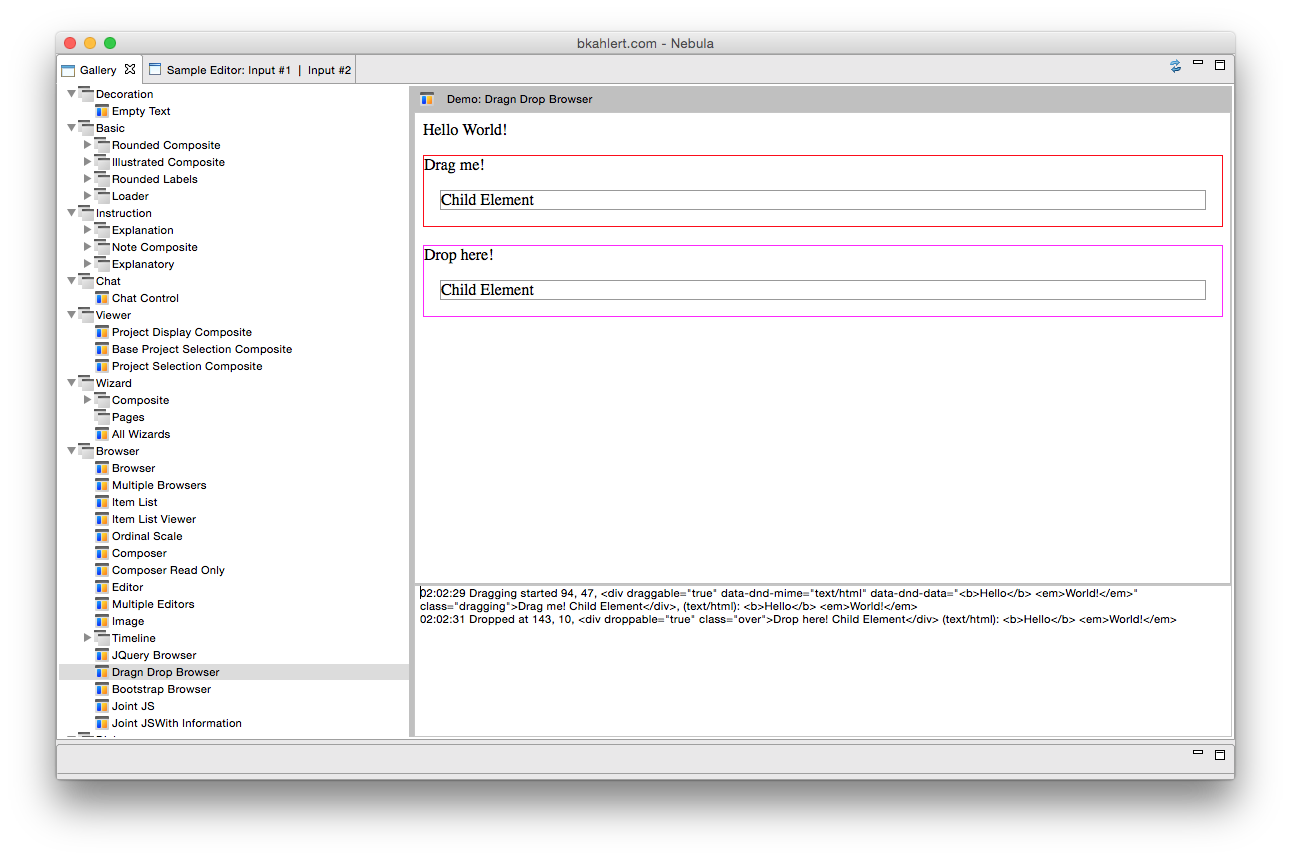
\includegraphics[width=1.0\linewidth]{Figures/browser/BrowserDND.png}
  \caption[Nebula-Browser: Drag'n'Drop]{Im rechten Bereich der \textit{Widget Gallery} wird die Drag'n'Drop-Funktionalität des \textit{Nebula}-Browsers demonstriert.}  \label{fig:BrowserDND}
\end{figure}

Implementiert wird ein Großteil der oben beschriebenen Funktionen durch ein zu Beginn des Ladevorgangs injizierten JavaScript-Codes, der eine große Anzahl an Ereignissen an die Java-seitige \textit{Nebula}-Browser-Komponente weiterleitet.
Das Fangen von Fehlern wiederum wird ermöglicht, indem sämtlicher von Java-Seite ausgeführter JavaScript-Code entsprechend gekapselt wird.




\section*{Schwerwiegendes Problem mit dem Editor für axiales Kodieren}
\label{app:acm-editor-problem}

Beim Endspurt für diese Arbeit --- genauer gesagt beim Generieren der \gls{gt} --- arbeitete ich mit meinem APIUA-internen, Browser-basierten Editor für axiales Kodieren. Technisch greife ich dabei auf die JavaScript-basierte JointJS-Bibliothek\footnote{\url{http://www.jointjs.com}} zurück. Diese verwendet wiederum SVG zum Zeichnen meiner Graphen.

Als ich meiner Theorie ein weiteres Konzept hinzugefügt hatte, reagierte APIUA nicht mehr. Ich musste APIUA neu starten und bei jedem Versuch, den problematischen Theoriegraphen zu öffnen, wiederholte sich das Problem. Ich konnte nicht mehr arbeiten.

Der Eclipse-Debugger gab darüber Aufschluss, dass der \texttt{main}-Thread nicht mehr terminierte und es sich um die Ausführung nativen Codes handelte. Für das Debuggen musste ich also in den Browser wechseln und kleinschrittig das Problem reproduzieren, indem ich im Browser den Graphen lud und unter den letzten 478 JavaScript-Aufrufen den finden musste, der das Versagen provozierte.

Es handelte sich um eine Anweisung zur Erzeugung einer Kante zwischen zwei Knoten. Aber auch hier gab die interne Konsole des Browsers keine Fehlermeldungen aus, sondern terminierte nicht mehr. Nach unzähligen Zyklen von Debuggen-Versuchen, Browser-Abstürzen und -Neustarts stellte ich fest, dass JointJS zur Positionierung von Kantenbezeichnern die Funktion \texttt{SVGPathElement.getTotalLength()} zur Berechnung der Kantenlänge nutzte. Leider verfügt diese Funktion über einen Defekt, der bei bestimmten Bezierkurven zum besagten Versagen führt, bekannt ist\footnote{u.a. \url{https://bugzilla.mozilla.org/show_bug.cgi?id=1044355}\\und \url{https://code.google.com/p/chromium/issues/detail?id=349873}} und bis dato nicht behoben wurde.

Ich konnte das Problem verifizieren. Bereits das bloße Verschieben einer der verbundenen Knoten um einen Pixel führte nicht mehr zum Versagen. Eine Lösung, die nicht in Frage kam, denn das Versagen hätte bei anderen Konstellationen erneut auftreten können.

Glücklicherweise ist JavaScript eine Prototypen-basierte Sprache, was die Möglichkeit gibt, Funktionen überschreiben zu können, ohne mit Vererbung arbeiten zu müssen. Dadurch konnte ich die defekte Funktion \texttt{SVGPathElement.getTotalLength} überschreiben, ohne sämtliche Aufrufe auf Seiten von JointJS anpassen zu müssen.

Die JavaScript-Bibliothek Raphaël\footnote{\url{http://raphaeljs.com}} besitzt ebenfalls eine Implementierung für die Berechnung von Längen beliebiger Kurven. Diese konnte ich verwenden, um die Funktion korrekt zu überschreiben, was das Problem löste --- mich jedoch Stunden und Nerven kostete.% (siehe Abbildungen \ref{fig:acm-editor-problem-a} und \ref{fig:acm-editor-problem-b}).

\begin{comment}
\begin{figure}
        \centering
        \begin{subfigure}{0.38\linewidth}
                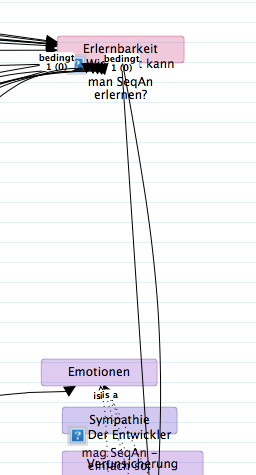
\includegraphics[width=\linewidth]{Figures/apiua/acm-editor-problem-a.png}
                  \caption[Axiales Kodieren Problem: ungelöst]{defekte Längenberechnung}
                \label{fig:acm-editor-problem-a}
        \end{subfigure}%
        \hfill%
        \begin{subfigure}{0.38\linewidth}
                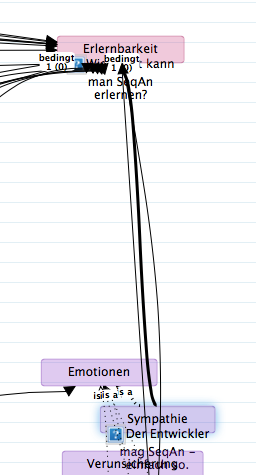
\includegraphics[width=\linewidth]{Figures/apiua/acm-editor-problem-b.png}
                  \caption[Axiales Kodieren Problem: gelöst]{korrigierte Längenberechnung}
                \label{fig:acm-editor-problem-b}
        \end{subfigure}%
        \caption[JointJS-Bug]{Vergleich der betroffenen Graphen}%
\end{figure}
\end{comment}